%!TEX root = ../04-Vakuum.tex
\chapter{Pyhsical Vapor Deposition}

A tantalum boat is used to evaporate a thin layer of indium onto a glass pane at different pressure levels.
The glass is shielded by a circular aperture which is placed \SI{\sim2}{\cm} below the glass.
\autoref{img:pvd} shows the glass plane with the indium film.

The dot that was deposited at a lower pressure has sharper edges, while the other dot is more spread out.
Free indium atoms that collide with gas molecules are deflected or oxidized.
This happens more frequently at higher pressures, so patterns get more washed out.

There is also a difference in the deposition rate.
At such low pressures, thermal conductivity is proportional to the pressure, so the boat does not get as hot and a higher heating current must be used.
As the deposition rate was more than an order of magnitude slower at the higher pressure, there is no point in comparing heating currents quantitatively.

\begin{figure}[b!]
	\centering
	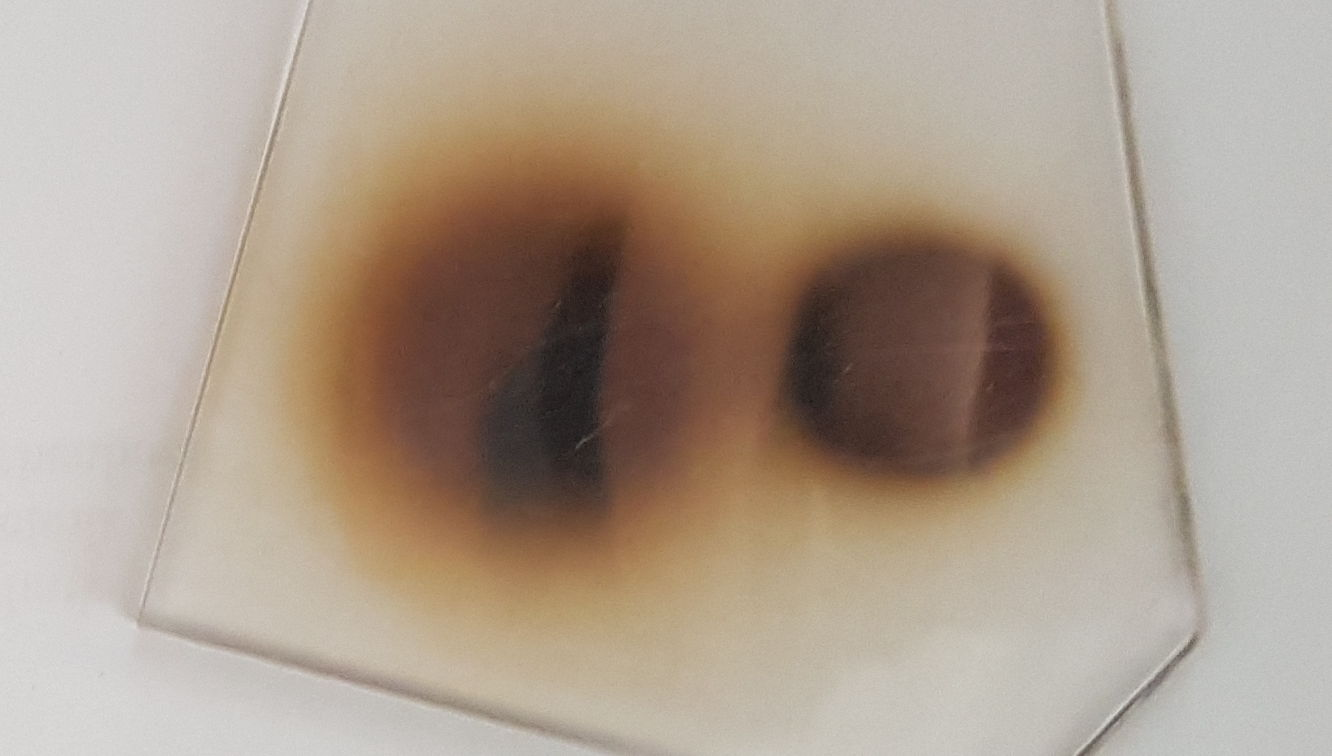
\includegraphics[width=.6\textwidth]{img/pvd.jpg}
	\caption[Indium Film]{Indium Film at \SI{e-2}{\milli\bar} (left) and \SI{e-4}{\milli\bar} (right)}
	\label{img:pvd}
\end{figure}
